\section*{Цель работы}

Углубленное изучение тиристора, исследование схемы
управляемого выпрямителя.



\section*{Исходные данные}

Все исследования, проводимые в лабораторной работе, выполняются с 
тиристором S4015L согласно 16 варианту.
Технические характеристики транзистора:

\begin{table}[h]
\centering
\caption{Технические характеристики тиристора S4015L}
\label{tab:datasheet}
\begin{tabular}{|c|c|c|}
\hline
\textbf{Символ} & \textbf{Значение} & \textbf{Единица измерения}\\
\hline
$V_{DRM}/V_{RRM}$ & 400 & В\\
\hline
$I_{TRMS}$ & 15 & A\\
\hline
$I_{H}$ & 40 & мА\\
\hline
\end{tabular}
\end{table}


\section*{Снятие ВАХ тиристора}

Для снятия ВАХ воспользуемся схемой на рисунке \ref{fig:вах_схема}.
Результат можно увидеть на рисунке \ref{fig:вах}. Для определения максимального
падения напряжения в рабочем режиме воспользуемся приближенным графиком на рисунке
\ref{fig:макс_пад_напр_в_раб_режиме}. Как видно, оно составляет около 1 В.

\begin{figure}[H]
    \centering
    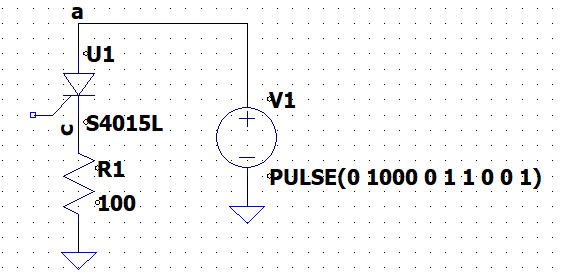
\includegraphics[width=0.8\textwidth]{figs/вах_схема.png}
    \caption{Схема для снятия ВАХ тиристора S4015L}
    \label{fig:вах_схема}
\end{figure}

\begin{figure}[H]
    \centering
    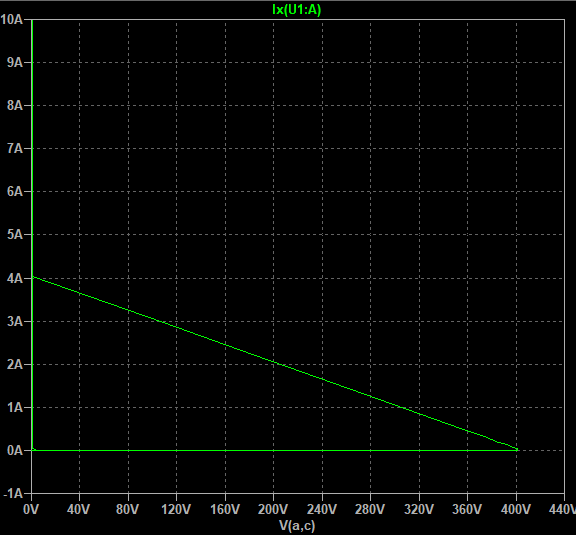
\includegraphics[width=0.8\textwidth]{figs/вах.png}
    \caption{ВАХ тиристора S4015L}
    \label{fig:вах}
\end{figure}

\begin{figure}[H]
    \centering
    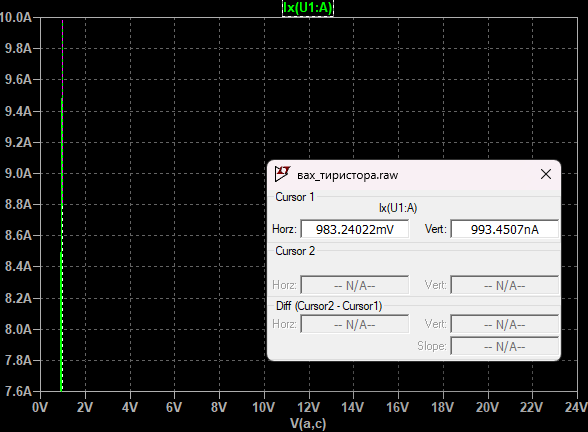
\includegraphics[width=0.8\textwidth]{figs/макс_пад_напр_в_раб_режиме.png}
    \caption{Максимальное падение напряжения в рабочем режиме около 1 В}
    \label{fig:макс_пад_напр_в_раб_режиме}
\end{figure}

\section*{Исследование работы однополупериодного управляемого
выпрямителя}

Был собран однополупериодный управляемый выпрямитель как на схеме на рисунке
\ref{fig:иссл_упр_выпр_схема}. Результаты, а именно входное, выходное
и управляющее напряжения, можно увидеть на рисунке \ref{fig:иссл_упр_выпр}.

Согласно симуляции среднее напряжение выхода составляет $34.753 V$, найдем его
аналитически по формуле:
\begin{equation*}
    U_{H_{\text{СР}}}=\frac{U_{2m}}{2\pi}(1+\cos\alpha)=\frac{110}{\pi}=35.014 V,
\end{equation*}
как видно, значения очень близки.

\begin{figure}[H]
    \centering
    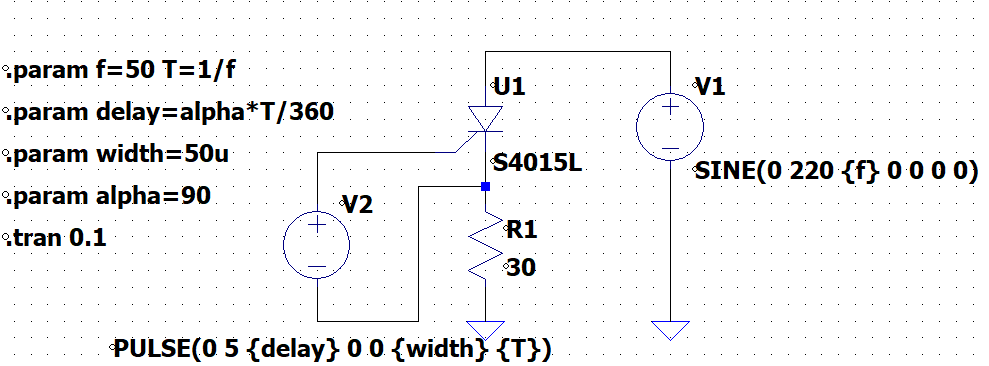
\includegraphics[width=0.8\textwidth]{figs/иссл_упр_выпр_схема.png}
    \caption{Схема для исследования работы однополупериодного
    управляемого выпрямителя}
    \label{fig:иссл_упр_выпр_схема}
\end{figure}

\begin{figure}[H]
    \centering
    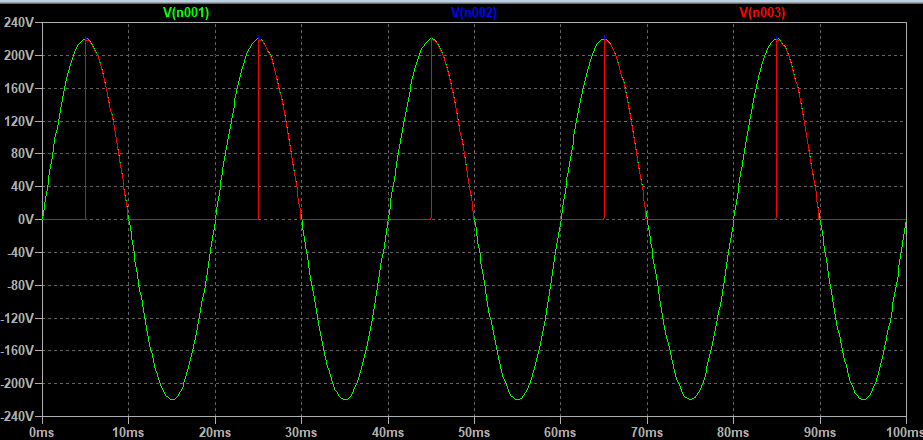
\includegraphics[width=1\textwidth]{figs/иссл_упр_выпр.png}
    \caption{Сигналы входного, выходного и управляющего напряжений в схеме 
    однополупериодного управляемого выпрямителя}
    \label{fig:иссл_упр_выпр}
\end{figure}

Снимим значения среднего напряжения на нагрузке для 10
значений угла включения тиристора $\alpha$ в диапазоне от 0
до 180 градусов (значения можно увидеть в таблице \ref{tab:средн_напр_на_нагрузке}). 
По полученным данным построена зависимость $U_{H_{\text{СР}}}=f(\alpha)$,
которую можно увидеть на рисунке \ref{fig:напр_ср_альфа}. С увеличением угла среднее
напряжение уменьшается, что ожидаемо, таким образом можно управлять мощностью на нагрузке.

\begin{table}[H]
    \centering
    \caption{Значения среднего напряжения на нагрузке}
    \label{tab:средн_напр_на_нагрузке}
    \begin{tabular}{|c|c|}
        \hline
        Угол ($\alpha$) & Среднее напряжение, В \\
        \hline
        18 & 67.900 \\
        36 & 62.962 \\
        54 & 55.263 \\
        72 & 45.533 \\
        90 & 34.753 \\
        108 & 23.977 \\
        126 & 14.263 \\
        144 & 6.563 \\
        162 & 1.635 \\
        180 & -0.008 \\
        \hline
    \end{tabular}
\end{table}

\begin{figure}[H]
    \centering
    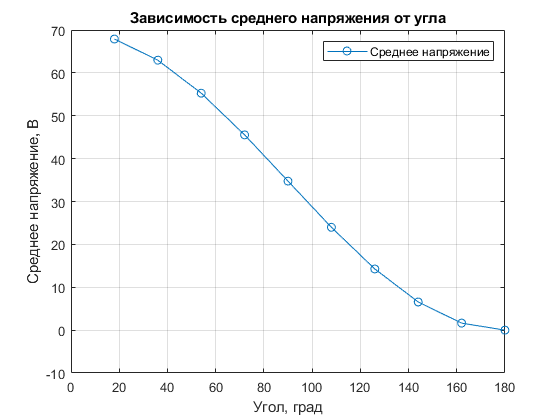
\includegraphics[width=0.8\textwidth]{figs/напр_ср_альфа.png}
    \caption{Зависимость среднего напряжения на нагрузке от угла}
    \label{fig:напр_ср_альфа}
\end{figure}

\newpage

\section*{Исследование работы однополупериодного регулятора
мощности}

Для реализации схемы тиристорного регулятора мощности дополним схему выпрямителя диодом
$RF2001T4S$ (см. схему на рисунке \ref{fig:иссл_мощ_схема}). Графики входного, выходного
и управляющего напряжений, можно увидеть на рисунке \ref{fig:иссл_мощ}.
Среднее напряжение на нагрузке согласно LTSpice составляет -34.825 В, найдем 
действующее напряжение на нагрузке по формуле:
\begin{equation*}
    U_{H_\text{Д}}=U_{2m}\sqrt{
        \frac{1}{8\pi}(4\pi-2\alpha-\sin(2\alpha))
    }=220\cdot\sqrt{\frac{1}{8\pi}(4\pi-\pi-\sin(\pi))}
    =134.7219 V.
\end{equation*}
Среднее значение и действующее значение напряжения сильно отличаюся.

\begin{figure}[H]
    \centering
    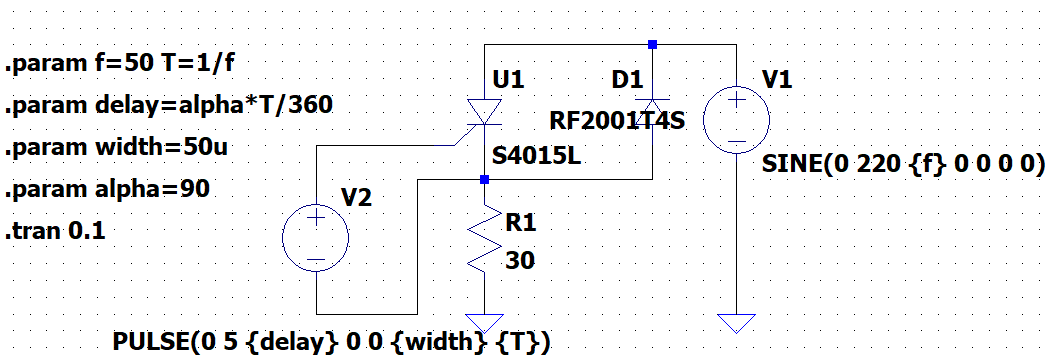
\includegraphics[width=0.8\textwidth]{figs/иссл_мощ_схема.png}
    \caption{Схема для исследования работы однополупериодного регулятора мощности}
    \label{fig:иссл_мощ_схема}
\end{figure}

\begin{figure}[H]
    \centering
    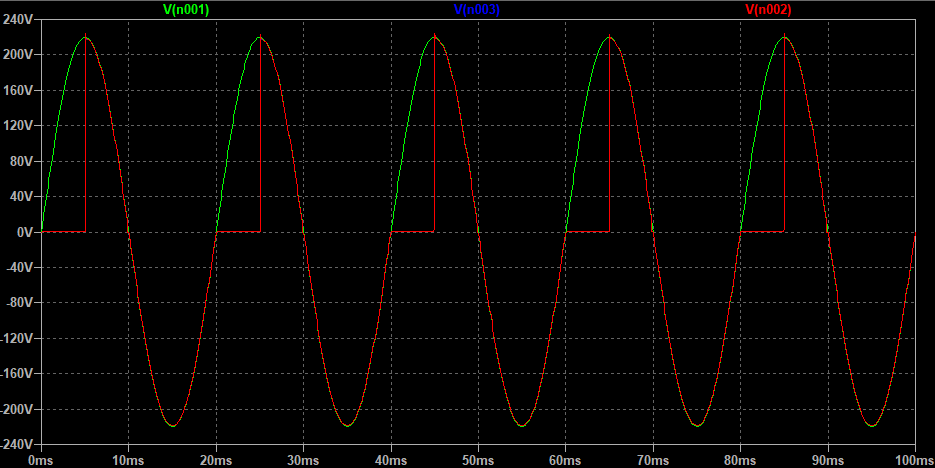
\includegraphics[width=1\textwidth]{figs/иссл_мощ.png}
    \caption{Сигналы входного, выходного и управляющего напряжений в схеме 
    однополупериодного регулятора мощности}
    \label{fig:иссл_мощ}
\end{figure}

Снимим значения среднего напряжения на нагрузке для 10
значений угла включения тиристора $\alpha$ в диапазоне от 0
до 180 градусов (значения можно увидеть в таблице \ref{tab:средн_напр_на_нагрузке_мощ}). 
По полученным данным построена зависимость $P_H=f(\alpha)$,
которую можно увидеть на рисунке \ref{fig:мощ_альфа}. Мощность вычислялась по формуле
\begin{equation*}
    P_H=\frac{220^2
        (4\pi-2\alpha-\sin(2\alpha))
    }{8\pi R_H}.
\end{equation*}
С увеличением угла средняя
мощность падает, что ожидаемо.


\begin{table}[H]
    \centering
    \caption{Значения среднего напряжения на нагрузке регулятора мощности}
    \label{tab:средн_напр_на_нагрузке_мощ}
    \begin{tabular}{|c|c|}
        \hline
        Угол ($\alpha$) & Среднее напряжение, В \\
        \hline
        18 & -0.0406 \\
        36 & -6.6179 \\
        54 & -14.3150 \\
        72 & -24.0460 \\
        90 & -34.8250 \\
        108 & -45.6010 \\
        126 & -55.3170 \\
        144 & -63.0130 \\
        162 & -67.9450 \\
        180 & -69.5770 \\
        \hline
    \end{tabular}
\end{table}

\begin{figure}[H]
    \centering
    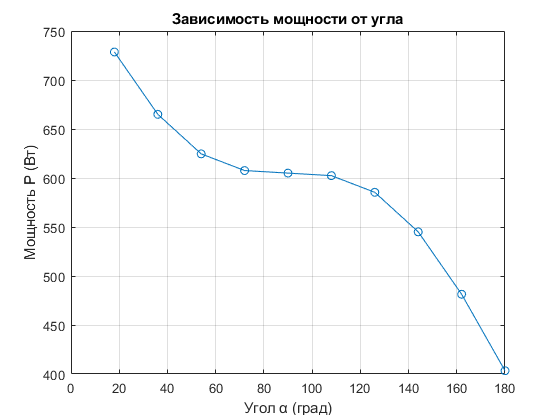
\includegraphics[width=0.8\textwidth]{figs/мощ_альфа.png}
    \caption{Зависимость мощности на нагрузке от угла}
    \label{fig:мощ_альфа}
\end{figure}


\section*{Заключение}

В ходе исследования схем однополупериодного управляемого
выпрямителя и однополупериодного регулятора
мощности были получены зависимости среднего напряжения и мощности
на нагрузке от угла включения тиристора, соответственно. При увеличении $\alpha$ среднее напряжение
как и мощность падали.
